\documentclass[cjk,slidestop,compress,mathserif,blue]{beamer}
%dvipdfm选项是关键,否则编译统统通不过
%beamer的颜色选项定义的是导航条和标题的颜色(即关键词structure的颜色)

%%%%%%%%%%%%%%%%仅限于XeTeX可使用的宏包%%%%%%%%%%%%%%%%%%%%%%%%%%%%
\usepackage{fontspec,xunicode,xltxtra,beamerthemesplit}
%\usepackage{beamerthemesplit}
\usepackage{xeCJK}
\setCJKmainfont[BoldFont=黑体, ItalicFont=楷体, BoldItalicFont=仿宋]{黑体}
%\setsansfont[Mapping=tex-text]{Adobe 黑体 Std}
%如果装了Adobe Acrobat,可在font.conf中配置Adobe字体的路径以使用其中文字体
%也可直接使用系统中的中文字体如SimSun,SimHei,微软雅黑 等
%原来beamer用的字体是sans family;注意Mapping的大小写,不能写错

%%%%%%%%   确定标题和导航条结构的框架     %%%%%%%%%%%%
\usepackage{beamerthemeshadow}                       %
%\usepackage{beamerthemeclassic}%导航条色与背景色一致%
%%%%%%%%%%%%%%%%%%%%%%%%%%%%%%%%%%%%%%%%%%%%%%%%%%%%%%
\setbeamerfont{roman title}{size={}}
%\usepackage{CJK} % CJK 中文支持                                  %
\usepackage{amsmath,amsthm,amsfonts,amssymb,bm}
\usepackage{mathrsfs}
\usepackage{xcolor}                                        %使用默认允许使用颜色
\usepackage{enumerate}                                     %使用标注数字
\usepackage{hyperref} 
\usepackage{graphicx}
\usepackage{subfigure}           %图片跨页
\usepackage{animate}		 %插入动画

%\usepackage[numbers,sort&compress]{natbib} %紧密排列             %
\usepackage[sectionbib]{chapterbib}        %每章节单独参考文献   %
\usepackage{hypernat}                                                                         %
%\usepackage[dvipdfm,bookmarksopen=true,pdfstartview=FitH,CJKbookmarks]{hyperref}		%
\hypersetup{bookmarksnumbered,colorlinks,linkcolor=brown,citecolor=blue,urlcolor=red}         %
%参考文献含有超链接引用时需要下列宏包,注意与natbib有冲突        %
%\usepackage[dvipdfm]{hyperref}                                  %
%\usepackage{hypernat}                                           %
\newcommand{\upcite}[1]{\hspace{0ex}\textsuperscript{\cite{#1}}} %

%\useoutertheme{smoothbars}
\useinnertheme[shadow=true]{rounded}
\usetheme{Berkeley}                                          %主题式样
%\usetheme{Luebeck}

\usecolortheme{lily}                                        %颜色主题式样

\usefonttheme{professionalfonts}                           %字体主题样式宏包

%\beamertemplatetransparentcoveredhigh                      %使所有被隐藏的文本高度透明
\beamertemplatetransparentcovereddynamicmedium             %使所有被隐藏的文本完全透明,动态,动态的范围很小
\mode<presentation>
%\beamersetaveragebackground{gray}                          %设置背景颜色(单一色) 
\beamertemplateshadingbackground{green!10}{red!5}         %设置背景颜色(渐变色)

%i放置单位logo
%\logo{
\includegraphics[width=1.6cm,height=0.35cm]{Figures/BCC_logo-1.png}}	%简单设置logo

%\pgfdeclareimage[width=3.5cm]{logoname}{Figures/BCC_logo-1.png}		%logo置于左侧微调
%\logo{\pgfuseimage{logoname}{\vspace{0.2cm}\hspace*{-2.0cm}}}

%在指定位置精确放置logo
\usepackage{tikz}
\usepackage{beamerfoils}
\usepackage{pgf}
\logo{\pgfputat{\pgfxy(11.68,0.15)}{
\includegraphics[height=1.01cm,viewport=0 0 140 120,clip]{Figures/BCC_logo-1.png}}\pgfputat{\pgfxy(10.502,-0.218)}{
\includegraphics[height=0.369cm,viewport=140 0 540 120,clip]{Figures/BCC_logo-1.png}}}
%\logo{\pgfputat{\pgfxy(11.68,0.15)}{
\includegraphics[height=0.95cm,viewport=0 0 510 360,clip]{Figures/Logo_Gainstrong.png}}\pgfputat{\pgfxy(10.333,-0.195)}{
\includegraphics[height=0.35cm,viewport=530 70 1100 218,clip]{Figures/Logo_Gainstrong.png}}}
%\MyLogo{
%	\pgfputat{\pgfxy(-50,-50)}{\pgfbox[right,base]{
\includegraphics[height=1cm]{Figures/BCC_logo-1.png}}}

%logo作为背景放置
%\setbeamertemplate{background}{
%	\pgfputat{\pgfxy(6.5,-0.5)}{\pgfbox[left,top]{\pgfimage[height=1.1cm]{Figures/BCC_logo-1.png}}}}

%\logo{}									%不显示logo

\begin{document}
%\begin{CJK*}{GBK}{song}
%\begin{CJK*}{GBK}{kai}
%beamer下不能用\songyi、\zihao等命令!
%\graphicspath{Figures/}

%-------------------------------PPT Title-------------------------------------
\title{\rm{Berry~}相位与极化}
%-----------------------------------------------------------------------------

%----------------------------Author & Date------------------------------------
\author{北京市计算中心\;云平台\:姜骏}
\date{\textrm{2016.12.28}}
%\date{2013.09.10}
\frame{\titlepage}
%-----------------------------------------------------------------------------

%------------------------------------------------------------------------------列出全文 outline ---------------------------------------------------------------------------------
\section*{}
\frame[allowframebreaks]
{
  \frametitle{Outline}
%  \frametitle{\textcolor{mycolor}{\secname}}
  \tableofcontents%[current,currentsection,currentsubsection]
}
%在每个section之前列出全部Outline
%类似的在每个subsection之前列出全部Outline是\AtBeginSubsection[]
\AtBeginSection[]
{
  \frame<handout:0>
  {
    \frametitle{Outline}
%全部Outline中,本部分加亮
    \tableofcontents[current,currentsection]
  }
}

%------------------------------------------------------------------------------PPT main Body------------------------------------------------------------------------------------
\small
\section{\rm{Wannier function}}
\frame
{
	\frametitle{\textrm{Wannier~}函数}
	\begin{itemize}
		\item \textrm{Wannier}函数是\textcolor{blue}{正交化的局域函数},\textcolor{red}{要求局域函数空间与能带空间完全相同}
		\item 紧束缚近似下,能带的电子波函数的\underline{\textcolor{blue}{\textrm{Bloch~}和}}
			\begin{displaymath}
				\psi_i^{\vec k}(\vec r)=\frac1{\sqrt N}\sum_m\mathrm{e}^{\mathrm{i}\vec k\cdot\vec R_m}\phi_i(\vec r-\vec R_m)
			\end{displaymath}
		\textrm{Bloch~}函数可以写类似形式
		\begin{displaymath}
			\psi_i^{\vec k}(\vec r)=\frac1{\sqrt N}\sum_m\mathrm{e}^{\mathrm{i}\vec k\cdot\vec R_m}W_i(\vec r-\vec R_m) 
		\end{displaymath}
		这里$W_i(\vec r-\vec R_n)$就是\textrm{Wannier~}函数
	\end{itemize}
}

\frame
{
	\frametitle{\textrm{Wannier~}函数}
	\begin{itemize}
		\item \textrm{Wannier~}函数是\textrm{Bloch~}函数的\textrm{Fourier}变换,对于格点$\vec T_m$有
			\begin{displaymath}
				\begin{aligned}
					&w_i(\vec r-\vec T_m)=\frac{\Omega_{\mathrm{cell}}}{2\pi^3}\int_{\mathrm{BZ}}\mathrm{d}\vec k\mathrm{e}^{-\mathrm{i}\vec k\cdot\vec T_m}\psi_i^{\vec k}(\vec r)\\
					=&\frac{\Omega_{\mathrm{cell}}}{2\pi^3}\int_{\mathrm{BZ}}\mathrm{d}\vec k\mathrm{e}^{-\mathrm{i}\vec k\cdot\vec T_m}\mathrm{e}^{-\mathrm{i}\vec k\cdot\vec r}u_i^{\vec k}(\vec r)=\frac{\Omega_{\mathrm{cell}}}{2\pi^3}\int_{\mathrm{BZ}}\mathrm{d}\vec k\mathrm{e}^{\mathrm{i}\vec k\cdot(\vec r-\vec T_m)}u_i^{\vec k}(\vec r)
				\end{aligned}
			\end{displaymath}
\begin{figure}[h!]
\centering
%\hspace*{-10pt}
\vspace*{-0.6in}
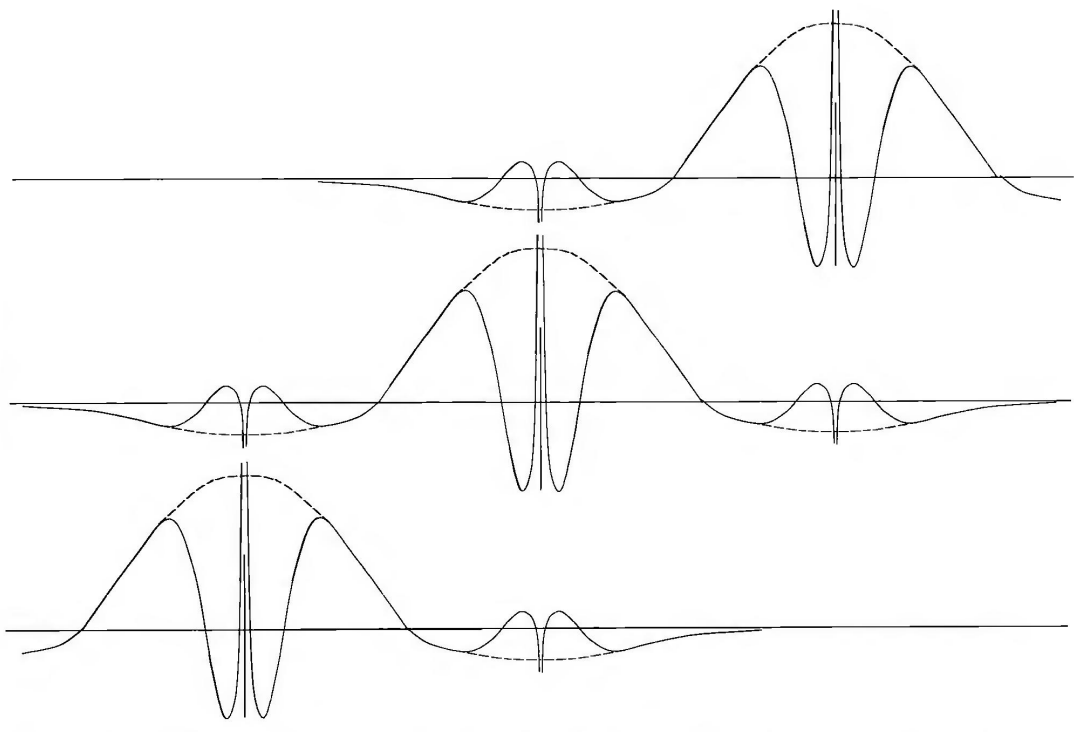
\includegraphics[height=1.8in,width=3.1in,viewport=0 0 1400 1000,clip]{Figures/Wannier_function.png}
\caption{\small \textrm{Schematic example of Wannier function that correspond to the Bloch function.}}%
\label{Wannier-function}
\end{figure} 
	\end{itemize}
}

\frame
{
	\frametitle{\textrm{Wannier~}函数}
	\begin{itemize}
		\item 一个能带的\textrm{Wannier~}函数完全由同一能带的\textrm{Bloch~}函数定义
		\item \textrm{Wannier~}函数完全正交
			\begin{displaymath}
				\int_{\textcolor{red}{\mathrm{all\; space}}}\mathrm{d}\vec rw_i^{\ast}(\vec r-\vec T_m)w_j(\vec r-\vec T_{m^{\prime}})=\delta_{ij}\delta_{mm^{\prime}}
			\end{displaymath}
			\textrm{Wannier~}函数和\textrm{Bloch~}函数一样,构成完备的正交函数集
		\item \textrm{Wannier~}函数间由幺正矩阵联系
			\begin{displaymath}
				u_{i\vec k}=\sum_jU_{ji}^{\vec k}u_{j\vec k}^{(0)}
			\end{displaymath}
			\textcolor{blue}{其中$U_{ji}^{\vec k}$是与$\vec k$~关联的幺正矩阵}
	\end{itemize}
}

\frame
{
	\frametitle{\textrm{Wannier~}函数的不唯一}
	\begin{itemize}
		\item 对于\textrm{Bloch~}函数
			\begin{displaymath}
				\psi_i^{\vec k}(\vec r)=\mathrm{e}^{\mathrm{i}\vec k\cdot\vec r}\mathrm{e}^{-\mathrm{i}\vec k\cdot\vec r}u_i^{\vec k}(\vec r)
			\end{displaymath}
			\textcolor{red}{可乘以任意相位,而不改变物理量的值}
			\begin{displaymath}
				\psi_i^{\vec k}(\vec r)\rightarrow\tilde\psi_i^{\vec k}(\vec r)=\textcolor{red}{\mathrm{e}^{\mathrm{i}\phi_i(\vec k)}}\psi_i^{\vec k}(\vec r)
			\end{displaymath}
		\item \textcolor{blue}{\textrm{Wannier~}函数的表示并不唯一}:\\
必须通过选择特定的相位$\phi_i(\vec k)$(或特定的幺正变换矩阵),才能得到确定的\textrm{Wannier~}函数 
\begin{figure}[h!]
\centering
%\hspace*{-10pt}
\vspace*{-0.3in}
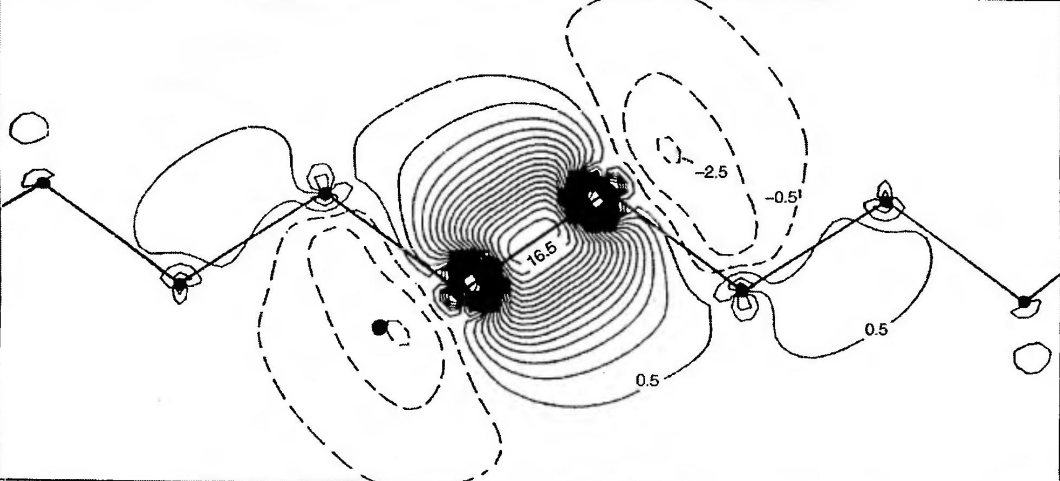
\includegraphics[height=1.1in,width=1.8in,viewport=0 0 1100 600,clip]{Figures/Wannier_function-Bondcenter_Si.png}
\caption{\small \textrm{Bond-centered Wannier function for Si.}}%
\label{Bond-Centered Wannier function}
\end{figure} 
	\end{itemize}
}

\frame
{
	\frametitle{\textrm{Wannier~}函数的不唯一}
\begin{figure}[h!]
\centering
\hspace*{-0.35in}
\subfigure[\textrm{Maximally localized Wannier function}]{
\label{Brillouin_Zone_Cubic}
\vspace*{-0.50in}
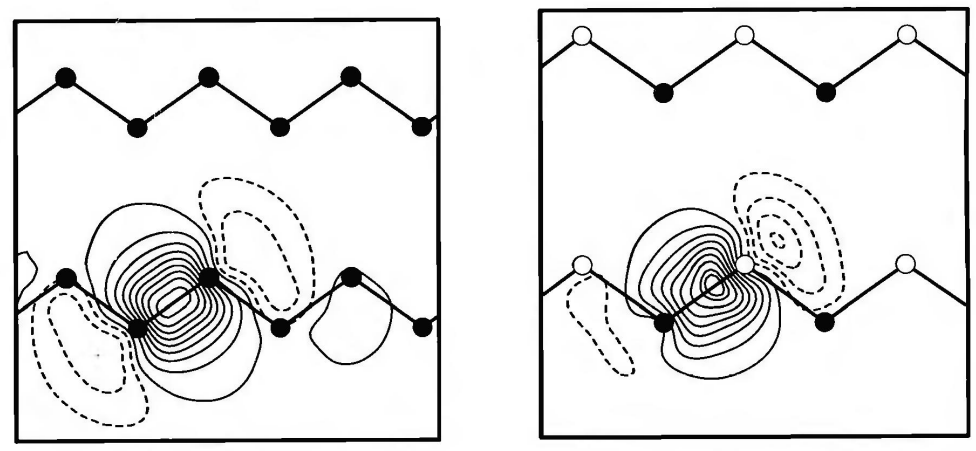
\includegraphics[height=1.10in,width=3.20in,viewport=0 0 1000 450,clip]{Figures/Wannier_function-Maxlocal.png}}
\subfigure[\textrm{Comparison of orthogonal and non-orthogonal maximally locaized orbitals}]{
\label{Band_Gap_SrSnO3}
\vspace*{-0.50in}
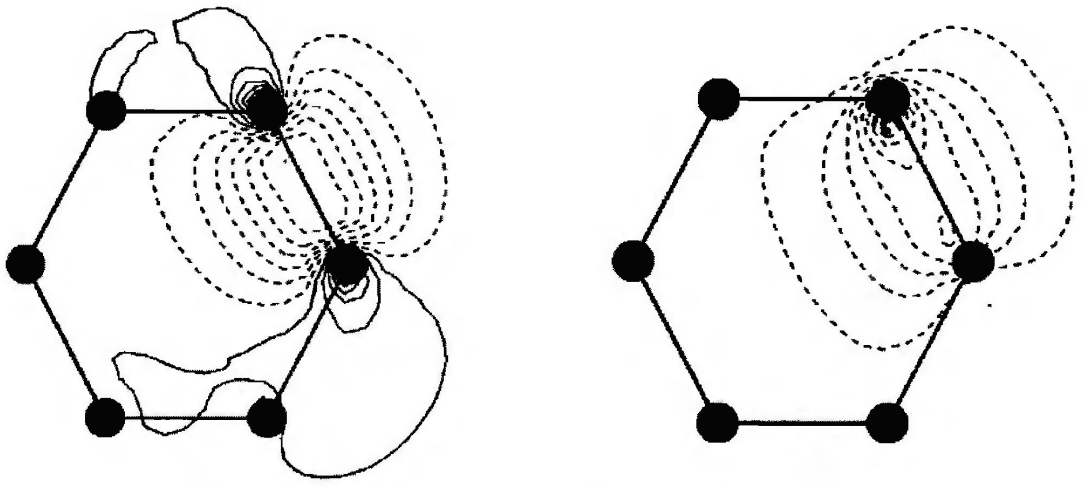
\includegraphics[height=1.10in,width=3.00in,viewport=0 0 1200 550,clip]{Figures/Non_orth-Wannier_function.png}}
\label{Non-local Wannier-function}
\end{figure}
}

\section{\rm{Berry~}相位}
\frame
{
	\frametitle{\textrm{Berry~}相位}
	\begin{itemize}
		\item 如果\textrm{Hamiltonian}依赖\textcolor{blue}{外部参数}$\vec R$:~$H(\vec R)$,有
	\begin{displaymath}
		H(\vec R)\psi_n(r;\vec R)=E_n(\vec R)\psi_n(r;\vec R)
	\end{displaymath}
	这里$r$是体系的\textcolor{blue}{内部变数}$\vec r$
		\item \textcolor{red}{讨论参数相关的本征态波函数的一般属性:}\\
			不同的参数$\vec R$不能唯一确定波函数$\psi_n(r;\vec R)$,因为波函数前乘任意与$\vec R$相关的相位角度,波函数模保持不变(标度不变)
		\item 假设$\psi_n(r;\vec R)$是在参数空间$D$范围内是连续、单值函数,引入标度的影响
			\begin{displaymath}
				\tilde\psi_n(r;\vec R)=\mathrm{e}^{\mathrm{i}\alpha_n(\vec R)}\psi_n(r;\vec R)
			\end{displaymath}
			这里相位角$\alpha_n(\vec R)$是连续、单值函数
	\end{itemize}
}

\frame
{
	\frametitle{\textrm{Berry~}相位}
\begin{figure}[h!]
\centering
%\hspace*{-10pt}
\vspace*{-0.2in}
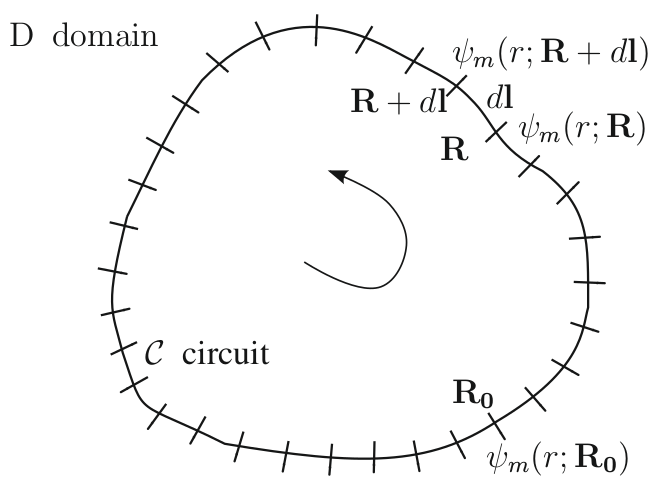
\includegraphics[height=1.1in,width=1.6in,viewport=0 0 650 500,clip]{Figures/Berry_Phase.png}
\caption{\small \textrm{Schematic representation of the sequence of states $\psi_n(r;\vec R)$ as $\vec R$ is changed along a circuit $C$ drawn in the parameter space $D$.}}%
\label{Berry_Phase}
\end{figure} 
如果在参数空间$\vec R$内有闭合回路$C$上有相邻两点$\vec R$和$\vec R+\mathrm{d}\vec I$,对应的本征态波函数为$\psi_m(r;\vec R)$和$\psi_m(r;\vec R+\mathrm{d}\vec I)$\\
\vskip 5pt
\textcolor{red}{这两个波函数的相位差$\mathrm{d}\phi$}
\begin{displaymath}
	\mathrm{d}\phi\equiv\arg\langle\psi_m(r;\vec R)|\psi_m(r;\vec R+\mathrm{d}\vec I)\rangle
\end{displaymath}
角度$\mathrm{d}\phi$表示了量子体系沿回路$C$绝热地由$\vec R$变化到$\vec R+\mathrm{d}\vec I$的相位变化,\textcolor{red}{因此$\mathrm{d}\phi$是标度相关的}
}

\frame
{
	\frametitle{\textrm{Berry~}相位}
	将$\psi_n(r;\vec R+\mathrm{d}I)$用\textrm{Taylor~}级数展开到一阶
	\begin{displaymath}
		\mathrm{d}\phi=\arg\left[ 1+\langle\psi_m(r;\vec R)|\frac{\partial}{\partial\vec R}\psi_m(r;\vec R)\rangle\cdot\mathrm{d}\vec I \right]
	\end{displaymath}
	\textcolor{red}{注意:~积分号内是纯虚数}
	\begin{displaymath}
		\mathrm{d}\phi=\Im\langle\psi_m(r;\vec R)|\frac{\partial}{\partial\vec R}\psi_m(r;\vec R)\rangle\cdot\mathrm{d}\vec I
	\end{displaymath}
	\textcolor{blue}{将闭合回路的几何角度$\gamma_m(C)$定义为\textrm{Berry~}相位}
	\begin{displaymath}
		\gamma_m(C)=\Im\oint_C\langle\psi_m(r;\vec R)|\frac{\partial}{\partial\vec R}\psi_m(r;\vec R)\rangle\cdot\mathrm{d}\vec I 
	\end{displaymath}
	将\textrm{Berry~}相位改为等价形式
	\begin{displaymath}
		\gamma_n(C)=\oint_C\mathbf{A}_n(\vec R)\cdot\mathrm{d}\vec I 
	\end{displaymath}
	其中$\mathbf{A}_n(\vec R)$定义为
%	\begin{displaymath}
	$\mathbf{A}_n(\vec R)=\Im\langle\psi_n(r;\vec R)|\nabla_{\vec R}\psi_n(r;\vec R)\rangle$
%	\end{displaymath}
}

\frame
{
	\frametitle{\textrm{Berry~}相位}
	\textcolor{red}{注意}:~几何相位$\gamma_n(C)$是\textcolor{blue}{标度不变的}\\
	虽然积分的每一步都是标度相关的
\begin{displaymath}
	\begin{aligned}
		\tilde{\mathbf{A}}_n(\vec R)=&\Im\langle\tilde\psi_n(r;\vec R)|\nabla_{\vec R}\tilde\psi_n(r;\vec R)\rangle\\
		=&\Im\langle\mathrm{e}^{\mathrm{i}\alpha_n(\vec R)}\psi_n(r;\vec R)|\nabla_{\vec R}\mathrm{e}^{\mathrm{i}\alpha_n(\vec R)}\psi_n(r;\vec R)\rangle\\
		=&\Im\langle\psi_n(r;\vec R)|\nabla_{\vec R}\psi_n(r;\vec R)\rangle+\nabla_{\vec R}\alpha_n(\vec R)
	\end{aligned}
\end{displaymath}
	因此
	\begin{displaymath}
		\tilde\gamma_n(C)=\oint_C\tilde{\mathbf{A}}_n(\vec R)\cdot\mathrm{d}\vec I=\oint_C[\mathbf{A}_n(\vec R)+\nabla_{\vec R}\alpha_n(\vec R)]\cdot\mathrm{d}\vec I\equiv\gamma_n(C)
	\end{displaymath}
	因为\textcolor{red}{对于闭合回路$\oint_C\nabla_{\vec R}\alpha_n(\vec R)\cdot\mathrm{d}\vec I=0$}\\
	\vskip 5pt
	利用\textrm{Stokes~}定理,可将闭合回路的积分变换成由围道$C$构成的表面积分
	\vskip -5pt
	\begin{displaymath}
		\gamma_n(C)=\oint_C\mathbf{A}_n(\vec R)\cdot\mathrm{d}\vec I=\int_S[\mathrm{curl}\mathbf{A}_n(\vec R)]\cdot\mathrm{d}\mathbf{S}
	\end{displaymath}
	\vskip -5pt
	注意到$\mathrm{curl}\mathbf{A}_n(\vec R)=\mathrm{curl}\tilde{\mathbf{A}}_n(\vec R)$
}

\frame
{
	\frametitle{\textrm{Berry~}相位}
	如果$\mathbf{B}_n(\vec R)$满足
	\begin{displaymath}
		\mathbf{B}_n(\vec R)=\mathrm{curl}\mathbf{A}_n(\vec R)
	\end{displaymath}
	利用基本关系
	\begin{displaymath}
		\hspace*{-15pt}
		\begin{aligned}
			\mathbf{B}_n(\vec R)=&\Im\,\mathrm{curl}\,\langle\psi_n(r;\vec R)|\nabla_{\vec R}\psi_n(r;\vec R)\rangle=\Im\,\langle\nabla_{\vec R}\psi_n(r;\vec R)|\times|\nabla_{\vec R}\psi_n(r;\vec R)\rangle\\
			=&\Im\sum_m\sideset{^{\prime}}{}\langle\nabla_{\vec R}\psi_n(r;\vec R)|\psi_m(r;\vec R)\rangle\times\langle\psi_m(r;\vec R)|\nabla_{\vec R}\psi_n(r;\vec R)\rangle
		\end{aligned}
	\end{displaymath}
	利用\textrm{Hellmann-Feynman~}定理
	\begin{displaymath}
		\hspace*{-10pt}
		\mathbf{B}_n(\vec R)=\Im\sum_m\sideset{^{\prime}}{}{}\frac{\langle\psi_n(r;\vec R)|\nabla_{\vec R}H|\psi_m(r;\vec R)\rangle\times\langle\psi_m(r;\vec R)|\nabla_{\vec R}H|\psi_n(r;\vec R)\rangle}{[E_n(\vec R)-E_m(\vec R)]^2}
	\end{displaymath}
	\textcolor{red}{注意:~$\mathbf{B}_n(\vec R)$是与波函数相位无关的物理量},并有
	\begin{displaymath}
		\gamma_n(C)=\int_S\mathbf{B}_n(\vec R)\mathrm{d}\mathbf{S}
	\end{displaymath}
	\textcolor{blue}{符合电磁场理论}
}

\section{现代极化理论与\rm{Berry~}相位}
\frame
{
	\frametitle{电介质材料的极化}
	\textcolor{blue}{电极化}:~电介质内部正负电荷的相对位移,会产生电偶极子,这现象称为电极化
	\begin{itemize}
\setlength{\itemsep}{10pt}
		\item \textcolor{red}{压电效应}:~\textcolor{blue}{电介质沿一定方向受外力发生形变时,内部会产生极化现象:~在电解质两个相对表面出现正负相反电荷;当作用力方向改变时,电荷的极性也随之改变;当外力去掉后,又会恢复到不带电的状态}
		\item \textcolor{red}{热电效应}:~\textcolor{blue}{电介质因为受热,电子(空穴)由高温区往低温区移动时,产生电荷堆积引起极化}
		\item \textcolor{red}{铁电效应}:~\textcolor{blue}{某些电介质中,晶胞的结构使正负电荷中心不重合而出现电偶极矩,在内部产生非零的电极化强度,使晶体具有自发极化,且电偶极矩方向可以因外电场而改变,呈现出类似于铁磁体的特点}
	\end{itemize}
}

\frame
{
	\frametitle{外电场下的极化}
	\begin{itemize}
		\item 金属在外电场下的极化
\begin{figure}[h!]
\centering
%\hspace*{-10pt}
\vspace*{-0.15in}
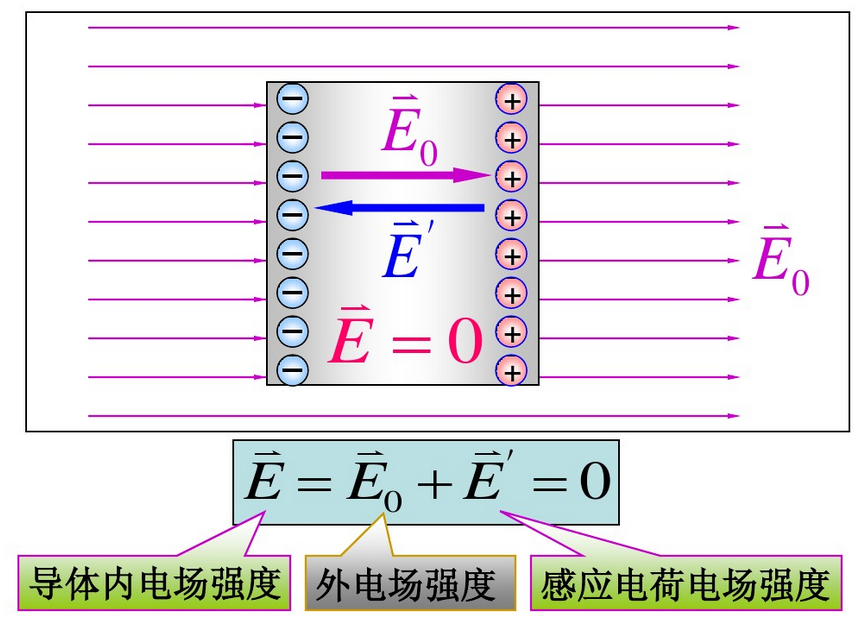
\includegraphics[height=1.8in,width=3.3in,viewport=0 0 1100 650,clip]{Figures/Polarize_metal-2.png}
\caption{\small \textrm{Schematic of a metal in the static electric field.}}%
\label{Polarization_metal}
\end{figure} 
\textcolor{blue}{金属体相的物理性质不会受外场的影响}
	\end{itemize}
}

\frame
{
	\frametitle{外电场下的极化}
	\begin{itemize}
		\item 绝缘体在外电场下的极化\\
			根据电磁理论,电场极化强度可定义为
			\begin{displaymath}
				\nabla\cdot\vec P(\vec r,t)=-\delta n(\vec r,t)
			\end{displaymath}
			利用极化电流守恒条件$\nabla\cdot\mathbf{j}(\vec r,t)=-\mathrm{d}n(\vec r,t)/\mathrm{d}t$\\
			可得电场极化强度与极化电流密度关系
			\begin{displaymath}
				\frac{\mathrm{d}\vec P(\vec r,t)}{\mathrm{d}t}=\mathbf{j}(\vec r,t)+\nabla\times\mathbf{M}(\vec r,t)
			\end{displaymath}
			这里$\mathbf{M}(\vec r,t)$是任意矢量场

			宏观电场极化强度一般定义为:\\\textcolor{blue}{单位体积中分子电偶极矩的矢量和}
	\end{itemize}
	\textcolor{red}{这样定义的极化强度存在一定的问题}
}

\frame
{
	\frametitle{外电场下的极化}
			\begin{enumerate}
				\item 对于有限体系,上述定义的电场极化强度是合理的
\begin{figure}[h!]
\centering
%\hspace*{-10pt}
\vspace*{-0.15in}
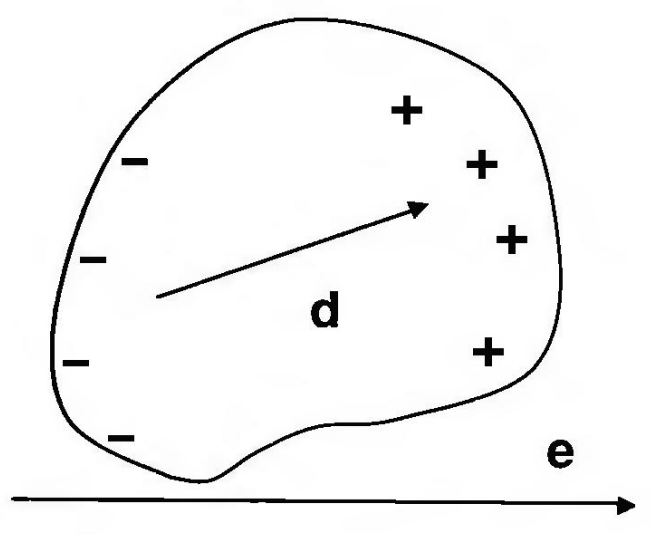
\includegraphics[height=0.9in,width=2.2in,viewport=0 0 1100 550,clip]{Figures/Polarize_insulator.png}
\caption{\small \textrm{Illustration of finite system for which the total dipole moment is well defined.}}%
\label{Polarization_insulator}
\end{figure} 
考虑到有限体系外$\vec P(\vec r)=0$,宏观电场极化强度$\vec P$可用偶极矩$\vec d$表示
\begin{displaymath}
	\vec P\equiv\frac{\vec d}{\Omega}=\frac1{\Omega}\int_{\mathrm{all\;space}}\mathrm{d}\vec rn(\vec r)\vec r
\end{displaymath}
\textcolor{red}{电场极化强度的变化$\Delta\vec P=\vec P^{(1)}-\vec P^{(0)}$只与电荷密度的改变$\Delta n=n^{(1)}-n^{(0)}$有关,而与电荷密度改变的路径有关}
			\end{enumerate}
}

\frame
{
	\frametitle{}
			\begin{enumerate}
				\setcounter{enumi}{1}
				\item 对于周期体系
\begin{figure}[h!]
\centering
%\hspace*{-10pt}
\vspace*{-0.15in}
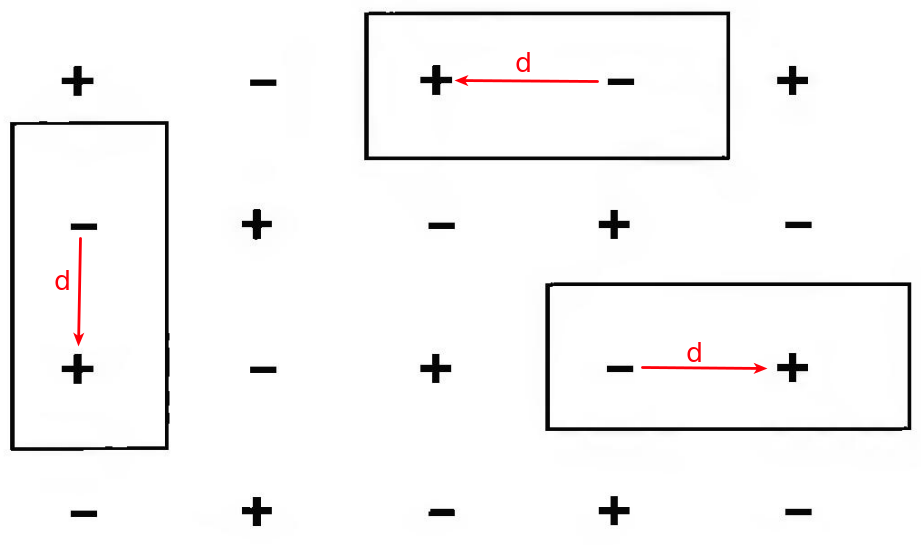
\includegraphics[height=0.9in,width=1.6in,viewport=0 0 1100 540,clip]{Figures/Polarize_insulator-2.png}
\caption{\small \textrm{Point charge model of an ionic crystal. The dipole is obviously not unique since the cells shown all have different moments.}}%
\label{Polarization_insulator-2}
\end{figure} 
正确定义周期体系的宏观电场极化强度,、\textcolor{red}{必须用合适的形式代替对$\vec r$的无限积分}\\
宏观极化电流是极化过程中唯一可观测的物理量,极化强度的变化$\vec P$可由体相极化电流计算
\begin{displaymath}
	\vec P(\vec r,t)=\int^t\mathrm{d}t^{\prime}\mathbf{j}_{\mathrm{int}}(\vec r,t^{\prime})
\end{displaymath}
			\end{enumerate}
}

\frame
{
	\frametitle{现代极化理论与几何\textrm{Berry~}相位}
	\begin{itemize}
		\item 用极化电流计算电场极化定义虽然正确,但不能证明电场极化强度与积分路径无关
		\item \textrm{King-Smith}和\textrm{Vanderbilt}提出了新的计算方案\upcite{PRB47-1651_1993}:\\
		\textcolor{red}{基本假设}:~连续的绝热变化可关联\textrm{Kohn-Sham}方程的\textrm{Hamiltonian}描述的不同态\\如果满足条件
	\begin{enumerate}
		\item 没有任何外部电场存在 
		\item 体系始终保持绝缘体状态
	\end{enumerate}
	宏观电场极化极化强度的变化可表示为
	\begin{displaymath}
		\Delta\vec P=\int_0^1\mathrm{d}\lambda\frac{\partial\vec P}{\partial\lambda}
	\end{displaymath}
	\textcolor{red}{注意}:~对所有的$\lambda$,宏观外电场要求为0
	\end{itemize}
}

\frame
{
	\frametitle{现代极化理论与几何\textrm{Berry~}相位}
	\begin{itemize}
		\item 根据线性响应理论,\textrm{Resta}指出:~在无限体系中,微扰项$\partial\vec P/\partial\lambda$可以用动量矩阵元表示\upcite{RMP66-899_1994}
	\begin{displaymath}
		\frac{\partial\vec P}{\partial\lambda}=-\mathrm{i}\frac{\mathrm{e}\hbar}{\Omega m_e}\sum_{\vec k}\sum_i^{\mathrm{occ}}\sum_j^{\mathrm{empty}}\frac{\langle\psi_{\vec k i}^{\lambda}|\hat{\vec p}|\psi_{\vec k j}^{\lambda}\rangle\langle\psi_{\vec k i}^{\lambda}|\partial V_{\mathrm{KS}}^{\lambda}/\partial\lambda|\psi_{\vec k j}^{\lambda}\rangle}{(\varepsilon_{\vec k i}^{\lambda}-\varepsilon_{\vec k j}^{\lambda})^2}+\mathrm{c.c.}
	\end{displaymath}
	这里对$i,j$的求和遍历所有自旋态
	\item 早先\textrm{Thouless}等在讨论量子\textrm{Hall~}效应时曾证明,上述对所有态的求和可变换成只对占据态的求和\upcite{PRL49-405_1982}\\引入与$\vec k$有关的\textrm{Kohn-Sham~}势$V_{\mathrm{KS}}^{(\lambda)}(\vec r)$,因此周期性\textrm{Hamiltonian~}表示为
	\begin{displaymath}
		\hat H(\vec k,\lambda)=\frac1{2m_e}\left( -\mathrm{i}\hbar\nabla+\hbar\vec k \right)^2+V_{\mathrm{KS}}^{(\lambda)}(\vec r)
	\end{displaymath}
	\end{itemize}
}

\frame
{
	\frametitle{现代极化理论与几何\textrm{Berry~}相位}
	利用\textrm{Bloch~}函数
	\begin{displaymath}
		\psi_{\vec k i}^{\lambda}=\mathrm{e}^{\mathrm{i}\vec k\cdot\vec r}u_{\vec k i}^{\lambda}(\vec r)
	\end{displaymath}
	满足等式
	\begin{displaymath}
		\hat H(\vec k,\lambda)u_{\vec k i}^{\lambda}(\vec r)=\left[ -\frac{\hbar}{2m_e}(\nabla+\mathrm{i}\vec k)^2 +V_{\mathrm{KS}}^{(\lambda)}(\vec r)\right]u_{\vec k i}^{\lambda}(\vec r)=\varepsilon_{\vec k i}^{\lambda}u_{\vec k i}^{\lambda}(\vec r)
	\end{displaymath}
	根据\textcolor{red}{对易关系}
	\begin{displaymath}
		\langle\psi_{\vec k i}^{\lambda}|\hat{\vec p}|\psi_{\vec k j}^{\lambda}\rangle=\frac{m_e}{\hbar}\langle u_{\vec k i}^{\lambda}|[\partial/\partial\vec k,\hat H(\vec k,\lambda)]|u_{\vec k j}^{\lambda}\rangle
	\end{displaymath}
	\begin{displaymath}
		\langle\psi_{\vec k i}^{\lambda}|\partial V_{\mathrm{KS}}^{\lambda}/\partial\lambda|\psi_{\vec k j}^{\lambda}\rangle=\frac{m_e}{\hbar}\langle u_{\vec k i}^{\lambda}|[\partial/\partial\lambda,\hat H(\vec k,\lambda)]|u_{\vec k j}^{\lambda}\rangle
	\end{displaymath}
	可得
	\begin{displaymath}
		\Delta\vec P_{\alpha}=-|e|\frac2{(2\pi)^3}\mathrm{Im}\int_{\mathrm{BZ}}\mathrm{d}\vec k\int_0^1\mathrm{d}\lambda\sum_i^{\mathrm{occ}}\left\langle\frac{\partial u_{\vec k i}^{(\lambda)}}{\partial k_{\alpha}}\right|\left.\frac{\partial u_{\vec k j}^{(\lambda)}}{\partial\lambda}\right\rangle
	\end{displaymath}
	对$\vec k$~的积分是倒空间的第一\textrm{Brillouin zone}
}

\frame
{
	\frametitle{现代极化理论和几何\textrm{Berry~}相位}
	\textrm{Thouless~}在讨论无相互作用粒子的量子\textrm{Hall~}效应时曾给出类似的积分表达式\upcite{PRB27-6083_1983},利用\textrm{Stokes~}定律
\begin{figure}[h!]
\centering
%\hspace*{-10pt}
\vspace*{-0.12in}
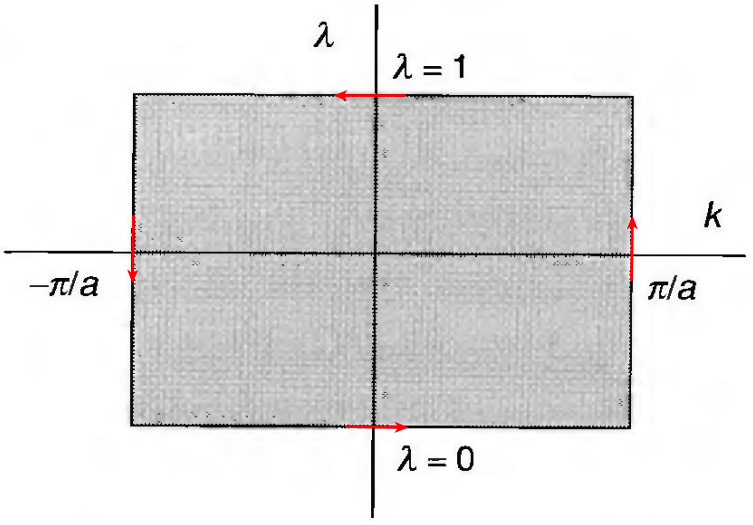
\includegraphics[height=1.2in,width=1.6in,viewport=0 0 800 540,clip]{Figures/Berry_contour_integration.png}
\caption{\small \textrm{Schematic figure of region of integration in $(k,\lambda)$ space for calculation of $\Delta P$ using the contour of integration C.}}%
\label{Berry_contour_integration}
\end{figure} 
	\begin{displaymath}
		\Delta P=-|e|\frac2{(2\pi)^3}\mathrm{Im}\sum_i^{\mathrm{occ}}\left\{ \underline{\textcolor{blue}{\oint_C\sum_{j=1}^2\mathrm{d}\tau_j\langle u_{k i}^{\lambda}|\partial/\partial\tau_j|u_{k i}^{\lambda}\rangle}} \right\} 
	\end{displaymath}
这里$\tau$~是二维空间$(\lambda,k)$,$C$是$\tau$空间的围道
}

\frame
{
	\frametitle{现代极化理论和几何\textrm{Berry~}相位}
	\begin{itemize}
		\item 上述大括号内的积分是\textcolor{red}{绝热近似下,利用周期波函数围道积分计算的\textrm{Berry~}相位改变}\upcite{PRS392-45_1984,PRL51-2167_1983}
		\item \textrm{Thouless~}指出上述围道积分对应的是在势$V_{\mathrm{KS}}^{(0)}=V_{\mathrm{KS}}^{(1)}$条件下的积分,\textcolor{blue}{围道积分计算的是实空间波函数点的相位变化}
		\item 考虑到波函数的周期性,用$(k,\lambda)$表示的相位变化可以加$2n\pi$而不变
	\end{itemize}
	利用周期函数$u_{\vec k i}^{(\lambda)}$的“周期标度关系”
	\begin{displaymath}
		u_{\vec k+\vec G i}^{(\lambda)}(\vec r)=\textcolor{green}{\mathrm{e}^{\mathrm{i}\vec G\cdot\vec r}}u_{\vec k i}^{(\lambda)}(\vec r)
	\end{displaymath}
	其中$\vec G$是倒空间格矢,因此这种标度关系并不唯一
%	选择$\vec G$满足在$\vec k$和$\vec k+\vec G$对$\lambda$的二重积分相互抵消,因此
	\begin{displaymath}
		\Delta\vec P_{\alpha}=\mathrm{i}\frac{-|e|}{(2\pi)^3}\sum_i^{\mathrm{occ}}\int_{\mathrm{BZ}}\mathrm{d}\vec k\left[ \langle u_{\vec k i}^{\lambda=1}|\partial/\partial_{k_{\alpha}}|u_{\vec k i}^{\lambda=1}\rangle-\langle u_{\vec k i}^{\lambda=0}|\partial/\partial_{k_{\alpha}}|u_{\vec k i}^{\lambda=0}\rangle \right]
	\end{displaymath}
}

\frame
{
	\frametitle{现代极化理论和几何\textrm{Berry~}相位}
	利用周期标度关系,可有
	\begin{displaymath}
		\Delta\vec P=\vec P^{(1)}-\vec P^{(0)}	
	\end{displaymath}
	其中
	\begin{displaymath}
		P_{\alpha}^{(\lambda)}=\mathrm{i}\frac{-|e|}{(2\pi)^3}\sum_i^{\mathrm{occ}}\int_{\mathrm{BZ}}\mathrm{d}\vec k\langle u_{\vec k i}^{(\lambda)}|\partial/\partial_{k_{\alpha}}|u_{\vec k i}^{(\lambda)}\rangle
	\end{displaymath}
	\textrm{Zak~}等指出,\textcolor{red}{上述表达式即能带$i$的\textrm{Berry~}相位}\upcite{PRL62-2747_1989,EPL18-239_1992}
	
	\textcolor{blue}{注意到\textrm{Wannier~}函数的形式与“周期标度”的相位密切相关},有
	\begin{displaymath}
		u_{\vec k i}^{(\lambda)}(\vec r)=\frac 1{\sqrt N}\sum_{\vec R}\mathrm{e}^{-\mathrm{i}\vec k\cdot(\vec r-\vec R)}w_i^{(\lambda)}(\vec r-\vec R)
	\end{displaymath}
	利用\textrm{Wannier~}函数,$P_{\alpha}^{(\lambda)}$可以具有更简单的形式
	\begin{displaymath}
		\vec P^{(\lambda)}=-\frac{2e}{\Omega}\sum_i^{\mathrm{occ}}\int\vec r|w_i^{(\lambda)}(\vec r)|^2\mathrm{d}\vec r
	\end{displaymath}
	这里$\Omega$是原胞体积
}

\frame
{
	\frametitle{现代极化理论和几何\textrm{Berry~}相位}
	\textcolor{red}{电介质的极化改变正比于由绝热变化引起的\textrm{Wannier~}函数的电荷中心的偏移}

	考虑到绝热变化要求$V_{\mathrm{KS}}^{(0)}=V_{\mathrm{KS}}^{(1)}$,因此周期函数$u_{\vec k i}^{(0)}$和$u_{\vec k i}^{(1)}$仅有相位的差别
	\begin{displaymath}
		u_{\vec k i}^{(1)}=\mathrm{e}^{\mathrm{i}\theta_{\vec k i}}u_{\vec k i}^{(\lambda)}
	\end{displaymath}
	因此
	\begin{displaymath}
		\Delta P_{\alpha}=-\frac{|e|}{(2\pi)^3}\sum_i^{\mathrm{occ}}\int_{\mathrm{BZ}}\mathrm{d}\vec k\partial\theta_{\vec k i}/\partial k_{\alpha}
	\end{displaymath}
	$\mathrm{e}^{\mathrm{i}\theta_{\vec k i}}$是$\vec k$的周期函数,最一般的相位表示$\theta_{\vec k i}=\beta_{\vec k i}+\vec k\cdot\vec R$,因此
	\begin{displaymath}
		\Delta\vec P=-\frac{2e}{\Omega}\sum_i^{\mathrm{occ}}\vec R_i
	\end{displaymath}
}

\frame
{
	\frametitle{现代极化理论和几何\textrm{Berry~}相位}
	\begin{itemize}
		\item \textcolor{blue}{原胞内极化强度的变化即$-(2e/\Omega)R$}
		\item 特别地,考虑由于晶格平移$V_{\mathrm{KS}^{(\lambda)}}(\vec r)=V_{\mathrm{KS}}^{(0)}(\vec r-\lambda\vec R)$\\
			引起极化$\Delta P$为
			\begin{displaymath}
				\Delta P=-\frac{2e}{\Omega}N_{\mathrm{occ}}\vec R
			\end{displaymath}
	\end{itemize}
	实际计算$\Delta\vec P$有一定的复杂性:~\textcolor{blue}{因为\textrm{Brillouin zone}有限$\vec k$点上的本征态\textrm{Blochl~}函数间没有相关系}\\
	为了回避此困难,采用以下策略
	\begin{itemize}
		\item 选定格矢$\vec G_{\lVert}$平行于倒空间原胞最短的格矢,沿该方向
			\begin{displaymath}
				\Delta P_{\lVert}=P_{\lVert}^{(1)}-P_{\lVert}^{(0)}
			\end{displaymath}
			并有
			\begin{displaymath}
				P_{\lVert}^{(\lambda)}=\mathrm{i}\frac{-|e|}{(2\pi)^3}\int_{\mathrm{A}}\mathrm{d}\vec k_{\bot}\sum_i^{\mathrm{occ}}\int_0^{|\vec G_{\lVert}|}\mathrm{d}k_{\lVert}\left\langle u_{\vec k i}^{(\lambda)}\right|\frac{\partial}{\partial k_{\lVert}}\left|u_{\vec k i}^{(\lambda)}\right\rangle
			\end{displaymath}

	\end{itemize}
}

\frame
{
	\frametitle{现代极化理论和几何\textrm{Berry~}相位}
	\begin{itemize}
		\item 为完成积分,$\vec k$~空间的布点离散方案设置如下
			\begin{enumerate}
				\item 垂直于$\vec G_{\lVert}$方向的2\textrm{D~}平面上,采用传统的\textrm{Monkhorst-Pack}布点
				\item 在$\vec k_{\lVert}$方向上离散$J$个$\vec k$点
\begin{displaymath}
	\vec k_j=\vec k_{\bot}+j\vec G_{\lVert}/J
\end{displaymath}
这里$j$的取值由0到$J-1$\\
由此得到
\begin{equation}
	\phi_J^{(\lambda)}(\vec k_{\bot})=\mathrm{Im}\left\{ \ln\prod_{j=0}^{J-1}\det(\langle u_{\vec k_j m}^{(\lambda)}|u_{\vec k_{j+1 n}}^{(\lambda)}\rangle) \right\}
	\label{eq:phase_angle}
\end{equation}
这里$u_{\vec k_J n}^{(\lambda)}=\mathrm{e}^{-\mathrm{i}\vec G_{\lVert}\cdot\vec r}u_{\vec k_0 n}^{(\lambda)}$\\
$n$和$m$遍历全部电子占据的价带
			\end{enumerate}
	\end{itemize}
}

\frame
{
	\frametitle{现代极化理论和几何\textrm{Berry~}相位}
	在$J\rightarrow\infty$极限条件下
	\begin{displaymath}
		\begin{aligned}
			\phi^{(\lambda)}(\vec k_{\bot})\equiv&\lim_{J\rightarrow\infty}\phi_J^{(\lambda)}(\vec k_{\bot})\\
			&=-\mathrm{i}\sum_{i}^{\mathrm{occ}}\int_0^{|G_{\lVert}|}\mathrm{d}k_{\lVert}\langle u_{\vec k i}^{(\lambda)}|\partial/\partial k_{\lVert}|u_{\vec k i}^{(\lambda)}\rangle
		\end{aligned}
	\end{displaymath}
	于是$P_{\lVert}^{(\lambda)}$可表示为
	\begin{displaymath}
		P_{\lVert}^{(\lambda)}=\mathrm{i}\frac{2|e|}{(2\pi)^3}\int_{\mathrm A}\mathrm{d}\vec k_{\bot}\phi^{\lambda}(\vec k_{\bot})
	\end{displaymath}
	由此可知式\eqref{eq:phase_angle}中波函数的乘积与相位选择无关:\\
	\textcolor{blue}{$u_{\vec k i}^{(\lambda)}$的相位改变}\textcolor{red}{引起$P_{\lVert}^{(\lambda)}$的相位角上增加改变$n\cdot2\pi$}
}

%\section{匀强电场下的电介质与\rm{Berry~}相位}
\frame
{
	\frametitle{匀强电场下的电介质}
	\begin{itemize}
		\item \textcolor{purple}{极化与波函数相位的关系深化了对密度泛函理论的基态密度与周期体系物性的认识}
		\item 为处理介质处于匀强电场下的问题,\textrm{Nunes}和\textrm{Gonze}发展出了结合现代极化理论和变分-微扰(\textrm{variation-perturbation})的计算方法\upcite{PRB63-155107_2001}
			\begin{enumerate}
				\item 将外加匀强电场作为微扰
				\item 假设微扰极化的占据能带仍可用\textrm{Berry~}相理论表示\\
					\textcolor{blue}{外加匀强电场虽然破坏了体系平移周期性,电荷密度仍保持体系周期性,\textrm{Berry~}相位由极化的周期波函数计算}
				\item 波函数用微扰展开到二阶或更高,用变分迭代计算介电响应函数
			\end{enumerate}
		\item 将\textrm{Berry~}相位用电子波函数级数展开,必须要作离散化\\
			\begin{enumerate}
				\item \textrm{DAPE}:~先对\textrm{Hamiltonian}作微扰推导,再离散化计算\textrm{Berry~}相位
				\item \textrm{PEAD}:~在场相关\textrm{Hamiltonian~}基础上先离散计算\textrm{Berry~}相位,再作微扰推导
			\end{enumerate}
	\end{itemize}
}
%\frame
%{
%\frametitle{LDA+$U$近似处理含$d$、$f$\,电子的重元素体系}
%对局域的$d$\,或$f$\,电子,用含\textrm{$U$}的模型\textrm{Hamiltonian}考虑$d$-$d$或$f$-$f$间相互作用(定域\textrm{Coulomb}相互作用\textrm{$U$})。%,离域的\textit{s}\,和\textit{p}\,电子的运动用\textrm{LDA}近似描述。
%\begin{itemize}
%\setlength{\itemsep}{10pt}
%	\item \textrm{LDA+$U$}方法最重要的特征:通过参数\textrm{$U$}校正\textrm{LDA}中的电子自相互作用,使单电子能量变化出现不连续。%计算表明LDA+U方法对含有定域强Coulomb相互作用的体系是有效的\upcite{PRB48-16929_1993,JPCS56-1521_1995,EPL36-551_1996}。无论
%	\item \textrm{LDA+$U$}方法是平均场近似,对含有近似芯层的局域4$f$\,电子的镧系元素离子还是过渡金属的氧化物(金属的3$d$\,电子与氧原子2$p$\,电子有很强的相互作用)体系都有效。如\textrm{FeSi}和\textrm{LaCaO$_3$}等体系,\textrm{LDA+$U$}能给出有关于金属-绝缘体转变的有用信息。甚至用于含有5$f$\,电子的化合物的研究也取得一定的成功。
%\end{itemize}
%}

\appendix
%------------------------------------------------------------------------Reference----------------------------------------------------------------------------------------------
%\begin{thebibliography}{99}
%-----------------------------------------------------------------------------------------------------------------------------------------------------------------------%
%\frame
%{
%\frametitle{主要参考文献}
%{\small
%\bibitem{Singh_Book}\textrm{D. J. Singh. \textit{Plane Wave, PseudoPotential and the LAPW method} (Kluwer Academic, Boston,USA, 1994)}					%
%  \nocite{*}																				%
%}
%}
%\end{thebibliography}
\begin{thebibliography}{99}
\frame
{
\frametitle{主要参考文献}
{\small
\fontsize{9.5pt}{3.9pt}\selectfont{
%	\bibitem{Huang_Han}黄昆\:原著、韩汝琦\:改编, {\textit{固体物理学}}\:高等教育出版社, 北京, 1988
%	\bibitem{Xie_Lu}谢希德、陆栋\:主编, {\textit{固体能带理论}}\:复旦大学出版社, 上海, 1998
	\bibitem{PRB47-1651_1993}\textrm{R. D. King-Simth and D. Vanderbilt, \textit{Phys. Rev.} B, \textbf{47} (1993), 1651}
	\bibitem{RMP66-899_1994}\textrm{R. Resta, \textit{Rev. Mod. Phys.} \textbf{66} (1994), 899}
	\bibitem{PRL49-405_1982}\textrm{D. J. Thouless, M. Kohmoto, M. P. Nightingale and M. den Nijs., \textit{Phys. Rev. Lett.} \textbf{49} (1982), 405}
	\bibitem{PRB27-6083_1983}\textrm{D. J. Thouless., \textit{Phys. Rev.} B, \textbf{27} (1983), 6083}
	\bibitem{PRS392-45_1984}\textrm{M. V. Berry., \textit{Proc. R. Soc.} London Ser. A \textbf{392} (1984), 45}
	\bibitem{PRL51-2167_1983}\textrm{B. Simon, \textit{Phys. Rev. Lett.}, \textbf{51} (1983), 2167}
	\bibitem{PRL62-2747_1989}\textrm{J. Zak, \textit{Phys. Rev. Lett.}, \textbf{62} (1989), 2747}
	\bibitem{EPL18-239_1992}\textrm{L. Michel and J. Zak., \textit{Europhys. Lett.}, \textbf{18} (1992), 239}
	\bibitem{PRB63-155107_2001}\textcolor{red}{\frame{\textrm{R. W. Nunes and X. Gonze., \textit{Phys. Rev.} B, \textbf{63} (2001), 155107}}}
	\bibitem{PRL73-712_1994}\textrm{R. W. Nunes and D. Vanderbilt., \textit{Phys. Rev. Lett.}, \textbf{73} (1994), 712}}
}
\nocite*{}
}
\end{thebibliography}

%{\small
%\phantomsection\addcontentsline{toc}{section}{Bibliography}	 %直接调用\addcontentsline命令可能导致超链指向不准确,一般需要在之前调用一次\phantomsection命令加以修正	%
%\bibliography{Myref}																			%
%\bibliographystyle{mybib}																		%
%  \nocite{*}																				%
%}
%-----------------------------------------------------------------------------------------------------------------------------------------------------------------------%


%-----------------------------------------------------------Beamer下不建议使用bib,因为涉及分页--------------------------------------------------------------------------%
%{\small
%\phantomsection\addcontentsline{toc}{section}{Bibliography}	 %直接调用\addcontentsline命令可能导致超链指向不准确,一般需要在之前调用一次\phantomsection命令加以修正	%
%\bibliography{Myref}																			%
%\bibliographystyle{mybib}																		%
%  \nocite{*}																				%
%}

%------------------------------------------------------------------------------------------------------------------------------------------------------------------------------%

%-------------------------------------------------------------------------Thanks------------------------------------------------------------------------------------------------
%\section{致谢}
%\frame
%{
%\frametitle{致$\quad$谢}
%\begin{itemize}
%    \setlength{\itemsep}{20pt}
%  \item 感谢本团队高兴誉、吴泉生、宋红州等各位老师参与的讨论
%  \item 感谢莫所长、宋主任以及软件中心各位老师和同事
%  \item 感谢王崇愚先生的帮助
%\end{itemize}
%}

\logo{}									%不显示logo
\frame
{
\vskip 60 pt
%\hskip 10pt \textcolor{blue}{\Huge 感谢答辩委员会各位老师\,\textrm{!}}\\
\vskip 35 pt
\hskip 60pt \textcolor{blue}{\Huge 谢谢大家\:!}
%\vskip 15 pt
%\hskip 40pt \textcolor{blue}{\Huge \textrm{for your attention\:!}}
}

%-------------------------------------------------------------------------------------------------------------------------------------------------------------------------------

\clearpage
%\end{CJK*}
\end{document}
